\documentclass{beamer}

\usepackage{textcomp}
% \usepackage{a4wide}
\usepackage{caption}
\usepackage{subfig}
\usepackage{listings}
\usepackage{hyperref}
\usepackage{pgfplots}
\usepackage{tikz}
\usepackage{amsthm}
\usepackage{pgf,pgfarrows,pgfnodes}

\usepackage[T2A]{fontenc} 
\usepackage{alltt}
\usepackage[english]{babel}
\usepackage{amsmath}
\usepackage{amsfonts}
\usepackage{amssymb}
\usepackage{wrapfig}
\usepackage{indentfirst}
\usepackage{setspace}
\usepackage{graphicx}
\usepackage{textcomp}
\usepackage{array}
\usepackage[utf8]{inputenc}

\newcommand{\GP}{\mathcal{GP}}
\newcommand{\E}{\mathbb{E}}
\newcommand{\R}{\mathbb{R}}
\newcommand{\N}{\mathcal{N}}
\newcommand{\cov}{\mbox{cov}}
\newcommand{\Nystrom}{Nystr\"{o}m }
\newcommand{\KL}[2]{\mbox{KL}\left(#1\mbox{ || }#2\right)}
\newcommand{\tr}{\mbox{tr}}
\newcommand{\derivative}[2]{\frac{\partial #1}{\partial #2}}
\newcommand{\sndderivative}[3]{\frac{\partial^2 #1}{\partial #2 \partial #3}}
\AtBeginSection{\frame{\sectionpage}}

% \newtheorem{definition}{Definition}
% \newtheorem{theorem}{Theorem}

\usetheme{Boadilla}
\usecolortheme{lily}
\title{Gaussian Processes for Machine Learning}
\author{P. Izmailov}
\date{April 15, 2016}
%\institute{Lomonosov Moscow State University}

\begin{document}
	\begin{frame}
		\maketitle
	\end{frame}
		\begin{frame}{Outline}
			\tableofcontents[pausesections]
		\end{frame}
	\section{Gaussian Process}
		\begin{frame}{Gaussian Process}
			\begin{definition}
				A Gaussian process is a collection of random variables, any finite number of which have a joint Gaussian distribution.
			\end{definition}

			$$f \sim \GP(m(\cdot), k(\cdot, \cdot)) \Leftrightarrow f(t_1, \ldots, t_n) \sim \N(\mu, K),$$
			where $\mu = (m(t_1), \ldots, m(t_n))^T$, $K \in \R^{n \times n}$, $K_{ij} = k(t_i, t_j)$.

			$m: \R \rightarrow \R$ is called the mean function of the gaussian process $f$.

			$k: \R \times \R \rightarrow \R_+$ is the covariance function of $f$.

			\vspace{0.5cm}
			Mean and covariance functions completely determine a gaussian process.

		\end{frame}

		\begin{frame}{Example}
			\begin{figure}[!h]
				\centering
				\subfloat{
					\scalebox{0.5}{
						\input{../../Code/Experiments/pictures/1dgp-regression_nodata.pgf}
					}
				}
				\subfloat{
					\scalebox{0.5}{
						\input{../../Code/Experiments/pictures/2dgp-regression_nodata.pgf}
					}
				}
				\caption{Examples of gaussian processes}
			\end{figure}
		\end{frame}

		\begin{frame}{Covariance functions}
			\begin{figure}[!h]
				\centering
				\subfloat{
					\scalebox{0.3}{
						\input{../../Code/Experiments/pictures/1dgp-regression_gamma_05.pgf}
					}
				}
				\subfloat{
					\scalebox{0.3}{
						\input{../../Code/Experiments/pictures/1dgp-regression_gamma_1.pgf}
					}
				}
				\subfloat{
					\scalebox{0.3}{
						\input{../../Code/Experiments/pictures/1dgp-regression_gamma_2.pgf}
					}
				}
				% \caption{Gamma-exponential covariance function, different $\gamma$}
			% \end{figure}

			% \begin{figure}[!h]
			% 	\centering
				% \\
				\subfloat{
					\scalebox{0.3}{
						\input{../../Code/Experiments/pictures/1dgp-regression_matern_01.pgf}
					}
				}
				\subfloat{
					\scalebox{0.3}{
						\input{../../Code/Experiments/pictures/1dgp-regression_matern_05.pgf}
					}
				}
				\subfloat{
					\scalebox{0.3}{
						\input{../../Code/Experiments/pictures/1dgp-regression_matern_1.pgf}
					}
				}
				\caption{Gamma-exponential and Matern covariance functions}
			\end{figure}
		\end{frame}
	\section{Gaussian Process Regression}
		\begin{frame}{Problem statement and notation}
			\begin{itemize}
				\item $\{(x_i, f_i) | i = 1, \ldots, n\}$ — dataset, considered to be generated from a Gaussian process $f \sim \GP(m(\cdot), k(\cdot, \cdot))$, let $x \in \R^d$. 
				\item $X \in \R^{n \times d}$ — the matrix, comprised of data points $x_1, \ldots, x_n$.
				\item $f \in \R^n$ — the vector of target values $f_1, \ldots, f_n$.

				\item $y \in \R^n$ — the noisy version of $f$: $y \sim \N(y | f, \sigma_n^2 I)$

				\item $X_* \in \R^{k \times d}$ — new (test) data points.

				\item $f_* \in \R^k$ — the desired vector of process values at new data points $X_*$.

				\item $K(X, X) \in \R^{n \times n}$ — the matrix, comprised of pairvise values of the covariance function $k(\cdot, \cdot)$ of the underlying process:
				$$K(X, X)_{ij} = k(x_i, x_j).$$

				\item $K(X, X_*) \in \R^{n \times k}$ — the matrix, defined similarly to the $K(X, X)$.

				\item $K(X_*, X) = K(X, X_*)$.
			\end{itemize}

			\vspace{0.3cm}
			We want to obtain the predictive distribution
			$$p(f_* | X_*, X, y).$$
		\end{frame}

		\begin{frame}{Noise-free case}
			Let us consider the noise-free case first:
			$$y = f.$$

			We put the following prior on our model: the data is generated from a zero-mean gaussian process with covariance function $k(\cdot, \cdot)$:

			$$f \sim \GP(0, k(\cdot, \cdot)).$$

			This prior is not limiting, because zero-mean prior does not imply a zero-mean predictive distribution.

			

		\end{frame}

		\begin{frame}{Noise-free case}

			As $f$ and $f_{*}$ are assumed to be generated from the same gaussian proces, we have the following joint distribution

			$$\left [ \begin{array}{c} f\\ f_* \end{array} \right ]
			\sim
			\N \left ( 0, \left [\begin{array}{cc} K(X, X) & K(X, X_*)\\ K(X_*, X) & K(X_*, X_*) \end{array} \right] \right ).
			$$

			Marginalizing this distribution, we obtain the predictive
			% $$f_* | X_*, X, f $$
			$$f_* | X_*, X, f \sim \N( \hat m, \hat K ),$$
			where 
			$$\E [f_* | f ] = \hat m = K(X_*, X) K(X, X)^{-1} f,$$
			$$\cov(f_* | f ) = \hat K = K(X_*, X_*) - K(X_*, X)K(X, X)^{-1}K(X, X_*).$$

			% \hspace{0.5cm}
			% The computational complexity of this method is defined by the complexity of inversing the $K(X, X)$ matrix, and thus the method scales as $O(N^3)$.
		\end{frame}

		\begin{frame}{Noisy case}
			In the noisy case, we have a slightly different model:
			$$y = f + \varepsilon,$$
			where $\varepsilon \sim \N(0, \sigma_n^2 I)$.

			We can then rewrite the joint distribution as
			$$\left [ \begin{array}{c} y\\ f_* \end{array} \right ]
			\sim
			\N \left ( 0, \left [\begin{array}{cc} K(X, X) + \sigma_n^2 I & K(X, X_*)\\ K(X_*, X) & K(X_*, X_*) \end{array} \right] \right ).
			$$
			Marginalizing it once again we obtain the predictive
			$$f_* | y \sim \N( \hat m, \hat K ),$$
			$$\E[f_* | y] = \hat m = K(X_*, X) (K(X, X) + \sigma_n^2 I)^{-1} y,$$
			$$\cov(f_* | y ) = \hat K = K(X_*, X_*) - K(X_*, X)(K(X, X) + \sigma_n^2 I)^{-1}K(X, X_*).$$


		\end{frame}

		\begin{frame}{Example}
			\begin{figure}[!h]
				\centering
				\subfloat{
					\scalebox{0.5}{
						\input{../../Code/Experiments/pictures/1dgp-regression_noopt.pgf}
					}
				}
			\end{figure}

			As we can see, the method struggles to explain the data. In order to deal with this problem, we can tweak the covariance function. The covariance functions usualy have a set of parameters, which we will refer to as covariance (or kernel) hyper-parameters. Varying these parameters, we can find a better model for the data.

		\end{frame}

		\begin{frame}{Marginal likelihood}
			In order to find the best set of kernel hyper-parameters, we maximize the marginal likelihood with respect to them. In the case of gaussian process regression, this likelihood is given by
			$$p(y) = \N(y| 0, K(X, X) + \sigma_n^2 I) = $$
			$$ = -\frac 1 2 y^{T} (K(X, X) + \sigma_n^2 I)^{-1} y - \frac 1 2 \log |K(X, X) + \sigma_n^2 I| - \frac n 2 \log 2 \pi.$$

			If $k(\cdot, \cdot)$ is a differentiable function of it's hyper-parameters (which is usually true), $p(y)$ also is, and can be maximized with gradient-based optimization methods.
		\end{frame}

		\begin{frame}{Example}

			\begin{figure}[!h]
				\centering
				\subfloat{
					\scalebox{0.5}{
						\input{../../Code/Experiments/pictures/1dgp-regression_noopt.pgf}
					}
				}
				\subfloat{
					\scalebox{0.5}{
						\input{../../Code/Experiments/pictures/1dgp-regression_opt.pgf}
					}
				}
				\caption{Predictive distribution before and after hyper-parameter adaptation}
			\end{figure}

			As we can see, after adaptation of kernel hyper-parameters, the method does a better job, explaining the data.
		\end{frame}

		\begin{frame}{Computational Complexity}
			The computational complexity of the gaussian process regression is determined by the complexity of inversing the $K(X, X)$ matrix, and thus scales as $O(n^3)$. This complexity makes the method unaplicable to big problems and thus approximate aproaches are needed.
		\end{frame}
	\section{Inducing Inputs}
		\begin{frame}{Inducing Inputs}
			The graphical model for the gaussian process regression looks like this.
			\begin{figure}[!h]
				\centering
				\subfloat{
					\scalebox{0.5}{
						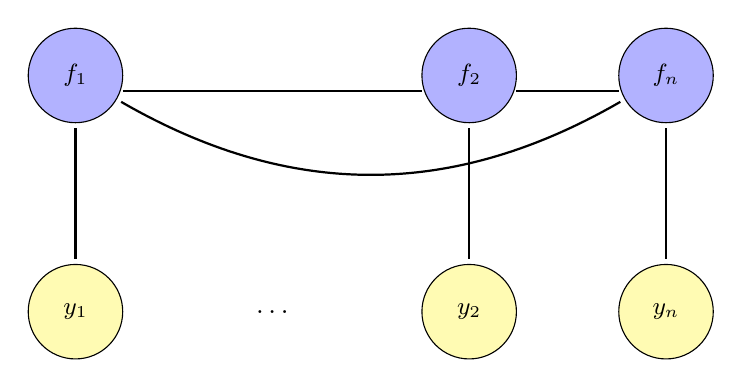
\begin{tikzpicture}
	\tikzstyle{x_i} = [circle, draw, fill=green!50, minimum size=1.2cm, text width=0.8cm, align=center, font=\large]
\tikzstyle{f_i} = [circle, draw, fill=blue!30, minimum size=1.2cm, inner sep=2pt, outer sep=2pt, font=\small, align=center]
\tikzstyle{y_i} = [circle, draw, fill=yellow!30, minimum size=1.2cm, inner sep=2pt, outer sep=2pt, font=\small, align=center]
\tikzstyle{edge_label} = [font=\small, label={[label distance = -4pt]90:$\text$}]
\tikzstyle{edge} = [thick, >=stealth]
\tikzstyle{biedge} = [thick, >=stealth]
\def\step{-3}
\def\layerpos{3}

% %data points
% \foreach \name/\x in {x_1/-2.5, x_2/2.5, x_n/5} 
%   	\node[x_i] (\name) at (\x, \layerpos) {$\name$};

% \node (other^1_1) at (0, \layerpos) {$\ldots$};

%latent process values
% \pgfmathsetmacro{\layerpos}{\layerpos + \step}

\foreach \name/\x in {f_1/-2.5, f_2/2.5, f_n/5} 
  	\node[f_i] (\name) at (\x, \layerpos) {$\name$};

% \node (other^2) at (0, \layerpos) {$\ldots$};
% \foreach \from/\to in {x_1/f_1, x_2/f_2, x_n/f_n}
% 	\draw[edge] (\from) -- (\to);

\draw[biedge] (f_1)++(0.6,-0.2) -- ++(3.8,0); %(f_2);
\draw[biedge] (f_2)++(0.6,-0.2) -- +(1.3,0);% ++ (f_n);
\draw [biedge] (f_1) to [out=-30,in=-150] (f_n);

%observables
\pgfmathsetmacro{\layerpos}{\layerpos + \step}

\foreach \name/\x in {y_1/-2.5, y_2/2.5, y_n/5} 
  	\node[y_i] (\name) at (\x, \layerpos) {$\name$};

\node (other^3) at (0, \layerpos) {$\ldots$};
\foreach \from/\to in {f_1/y_1, f_2/y_2, f_n/y_n}
	\draw[edge] (\from) -- (\to);
\end{tikzpicture}


					}
				}
			\end{figure}
		\end{frame}

		\begin{frame}{Inducing Inputs}
			Now we slightly change the model, adding a set of latent variables $u$.
			\begin{figure}[!h]
				\centering
				\subfloat{
					\scalebox{0.5}{
						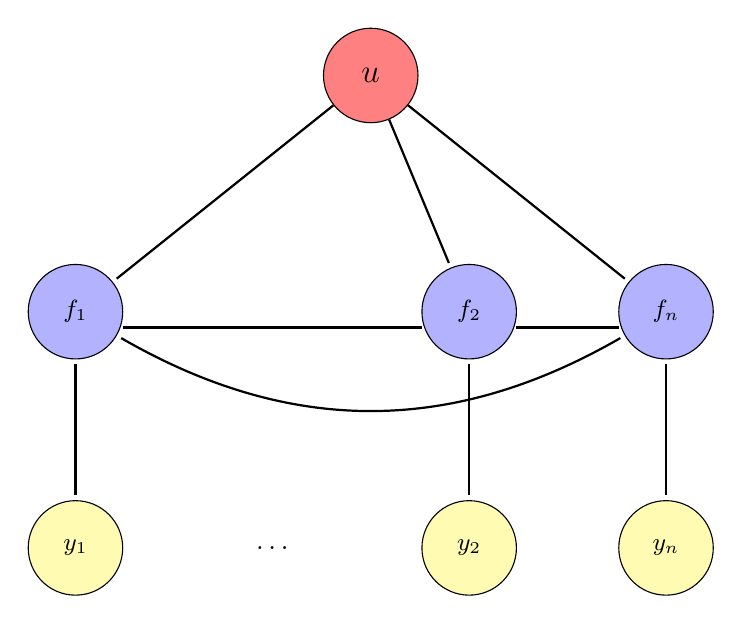
\begin{tikzpicture}
	\tikzstyle{u} = [circle, draw, fill=red!50, minimum size=1.2cm, text width=0.8cm, align=center, font=\large]
	\tikzstyle{x_i} = [circle, draw, fill=green!50, minimum size=1.2cm, text width=0.8cm, align=center, font=\large]
\tikzstyle{f_i} = [circle, draw, fill=blue!30, minimum size=1.2cm, inner sep=2pt, outer sep=2pt, font=\small, align=center]
\tikzstyle{y_i} = [circle, draw, fill=yellow!30, minimum size=1.2cm, inner sep=2pt, outer sep=2pt, font=\small, align=center]
\tikzstyle{edge_label} = [font=\small, label={[label distance = -4pt]90:$\text$}]
\tikzstyle{edge} = [thick, >=stealth]
\tikzstyle{biedge} = [thick, >=stealth]
\def\step{-3}
\def\layerpos{3}

% %data points
% \foreach \name/\x in {x_1/-2.5, x_2/2.5, x_n/5} 
%   	\node[x_i] (\name) at (\x, \layerpos) {$\name$};

% \node (other^1_1) at (0, \layerpos) {$\ldots$};

%latent process values
% \pgfmathsetmacro{\layerpos}{\layerpos + \step}

\foreach \name/\x in {f_1/-2.5, f_2/2.5, f_n/5} 
  	\node[f_i] (\name) at (\x, \layerpos) {$\name$};

% \node (other^2) at (0, \layerpos) {$\ldots$};
% \foreach \from/\to in {x_1/f_1, x_2/f_2, x_n/f_n}
% 	\draw[edge] (\from) -- (\to);

\draw[biedge] (f_1)++(0.6,-0.2) -- ++(3.8,0); %(f_2);
\draw[biedge] (f_2)++(0.6,-0.2) -- +(1.3,0);% ++ (f_n);
\draw [biedge] (f_1) to [out=-30,in=-150] (f_n);

%observables
\pgfmathsetmacro{\layerpos}{\layerpos + \step}

\foreach \name/\x in {y_1/-2.5, y_2/2.5, y_n/5} 
  	\node[y_i] (\name) at (\x, \layerpos) {$\name$};

\node (other^3) at (0, \layerpos) {$\ldots$};
\foreach \from/\to in {f_1/y_1, f_2/y_2, f_n/y_n}
	\draw[edge] (\from) -- (\to);
	\pgfmathsetmacro{\layerpos}{\step/2}
	\node[u] (inputs) at (1.25, 6) {$u$};

	\foreach \to in {f_1, f_2, f_n}
		\draw[edge] (inputs) -- (\to);
\end{tikzpicture}


					}
				}
			\end{figure}
			The joint probability of latent and observable variables now is given by
			$$p(y, f, u) = p(y | f) p(f | u) p(u).$$
		\end{frame}

		\begin{frame}{Inducing Inputs}
			The latent variables $u$ are referred to as inducing inputs. The intuition behind them is that they are considered as the values of the process at new data points $z_1, \ldots, z_m$. We will have to introduce some more notation now.

			\begin{itemize}
				\item $Z_m \in \R^{m \times d}$ — the matrix, comprised of the coordinates of the inducing inputs inputs $z_1, \ldots, z_m$.
				\item $K_{nn} = K(X, X)$
				\item $K_{mm} = K(Z_m, Z_m)$
				\item $K_{mn} = K(Z_m, X)$
				\item $K_{nm} = L(X, Z_m) = K_{mn}^T$ 
			\end{itemize}
			As $u_i$ are considered to be generated from the same gaussian process, as $f_i$, we have the following formulas.
			$$p(u) = \N(u|0, K_{mm}),$$
			$$p(f|u) = \N (f|K_{nm} K_{mm}^{-1}u, \tilde K),$$
			where $\tilde K = K_{nn} - K_{nm} K_{mm}^{-1} K_{mn}.$
		\end{frame}

		\begin{frame}{Evidence Lower Bound}
			The standard variational lower bound for the marginal likelihood $p(y)$ for our augmented model is
			$$p(y) \ge \E_{q(u, f)} \log \frac {p(y, u, f)}{q(u, f)} = \E_{q(u, f)} p(y | f) - \KL{q(u, f)} {p(u, f)}.$$

			Our model implies $\E_{q(u, f)} p(y | f) = \E_{q(f)} p(y | f)$, where $q(f)$ is the marginal of $q(u, f)$.

			We will consider the variational distributions of the following form:
			$$q(u, f) = p(f | u) q(u),$$
			where $q(u) \sim \N(u|\mu, \Sigma)$. This implies $q(f)$
			$$q(f) = \int p(u | f) q(u) du = $$
			$$\N(f| K_{nm} K_{mm}^{-1} \mu, K_{nn} + K_{nm} K_{mm}^{-1}(\Sigma - K_{mm}) K_{mm}^{-1} K_{mn}).$$
		\end{frame}

		\begin{frame}{Evidence Lower Bound}
			Now, consider the KL-divergence in the lower bound we've devised.
			$$\KL{q(u, f)} {p(u, f)} = \KL{q(u) p(f|u)} {p(u) p(f|u)} = \KL{q(u)} {p(u)}.$$

			Finally, the lower bound is
			$$p(y) \ge \E_{q(f)} p(y | f) + \KL{q(u)} {p(u)}.$$

			Note, that although, we've devised this bound for the regression problem, we never used the fact, that we are actually performing regression. This bound holds for binary classification problem as well.

			However, in the case of GP-regression, the right-hand side of the bound can be computed analytically in a closed form.
		\end{frame}

		\begin{frame}{SVI method}
			Substituting the normal distributions $q(u)$, $p(u)$, $q(f)$ and $p(y|f)$ back into the lower bound, we obtain the following inequality.
			$$p(y) \ge \sum_{i = 1}^{n} \left( \log \N(y_i | k_i^T K_{mm}^{-1} \mu, \sigma_n^2) - \frac 1 {2 \sigma_n^2} \tilde K_{ii} - \frac 1 2 \tr (\Sigma \Lambda_i) \right) - $$
			$$ -\frac 1 2 \left (\log \frac {|K_{mm}|} {|\Sigma|} - m + \tr(K_{mm}^{-1} \Sigma) + \mu^T K_{mm}^{-1} \mu \right),$$
			where $\Lambda_i = \frac 1 {\sigma_n^2} K_{mm}^{-1} k_i k_i^T K_{mm}^{-1}$, and $k_i$ is the $i$-th column of the matrix $K_{mn}$.

			This lower can be maximized with respect to kernel hyper-parameters and variational parameters $\mu, \Sigma$ using the stochastic optimization techniques. The authors of the method sudgest using the stochastic gradient descent with natural gradients for variational parameters. The complexity of computing a stochastic update for one object is $O(m^3)$.
		\end{frame}

		\begin{frame}{Titsias's method}
			The lower bound we devised can also be maximized with respect to variational parameters analytically. The optimal distribution $q^*(u) \sim \N(u|\hat u, \Lambda^{-1})$, where
			$$\Lambda = \frac 1 {\sigma_n} K_{mm}^{-1} K_{mn} K_{nm} K_{mm}^{-1} + K_{mm}^{-1},$$
			$$\hat u = \frac 1 {\sigma_n} \Lambda^{-1} K_{mm}^{-1} K_{mn} y.$$
			Substituting this distribution back to the ELBO, we obtain
			$$p(y) \ge -\frac 1 2 \left(n \log 2\pi + \log |B| + y^T B^{-1} y + \frac 1 {\sigma_n^2} \tr(\tilde K)\right),$$
			where $B = \sigma_n^2 I + K_{nm} K_{mm}^{-1} K_{mn}$. The complexity of computing the optimal distribution parameters, the lower bound and it's gradients is $O(n m^2)$. However, we can not apply stochastic optimization in this case.
		\end{frame}

		\begin{frame}{Example}
			\begin{figure}[!h]
				\centering
				\subfloat{
					\scalebox{0.5}{
						\input{../../Code/Experiments/pictures/1dgp-regression_means.pgf}
					}
				}
				\subfloat{
					\scalebox{0.5}{
						\input{../../Code/Experiments/pictures/1dgp-regression_vi.pgf}
					}
				}
				\caption{Example of two implementations of the Titsias's method. The \lstinline{vi} method maximizes the lower bound with respect to the positions of inducing inputs, while the \lstinline{means} method just uses the K-means cluster centers as inducing point positions.}
			\end{figure}
		\end{frame}



\end{document}
